\documentclass[a4paper, 11pt]{article}
\usepackage{comment} % enables the use of multi-line comments (\ifx \fi) 
\usepackage{lipsum} %This package just generates Lorem Ipsum filler text. 
\usepackage{fullpage} % changes the margin
\usepackage{hyperref}
\usepackage{graphicx}

\begin{document}
%Header-Make sure you update this information!!!!
\noindent
\large\textbf{Assignment 3} \hfill \textbf{Tyler Wilding} \\
\normalsize COSC 4426 \hfill Due Date: 02/10/16 \\
Prof. Biocchi \hfill No Source Code \\
TA: -- \hfill No Website

\section*{Packet Capturing}
Packet capturing is very useful and not used for just gathering sensitive information, it is also used for testing many things that are networking related.  As data is transferred amongst the network, the software picks up and logs the information and could even potentially decode it to show it in a more human readable format.  This can especially be used to see how the data is while in motion, if it is encrypted or not, if it is being intercepted along the way.

\section*{ARP Poisoning}
However, one of the issues when trying to capture packets in this assignment is that just simply looking at the packets on even a public WiFi with no encryption will not allow you to intercept information with just simple packet capturing software like wireshark.  This is because networks are much more complex now, information is not sent directly between clients for the most part, instead data first travels to the router or switch which will redirect the data to its final destination or to the next hop.  The router is not going to broadcast the information out to everyone on the network, only the relevant people.  However, this might also be due to the limiting nature of wireless cards on laptops and phones.\\

This is where ARP (Address Resolution Protocol) poisoning comes in handy.  This is a man in the middle attack that allows you to spoof to addresses in the network that you are the actual router.  No one else in the network as a user sees a noticable difference, the packets are simple transferred to your computer first and then to the router, hence the man in the middle attack.  Now that you have all packets going through your device you can use a program like wireshark to capture them.\\

We can actually see the arp poison in action through wireshark.\\
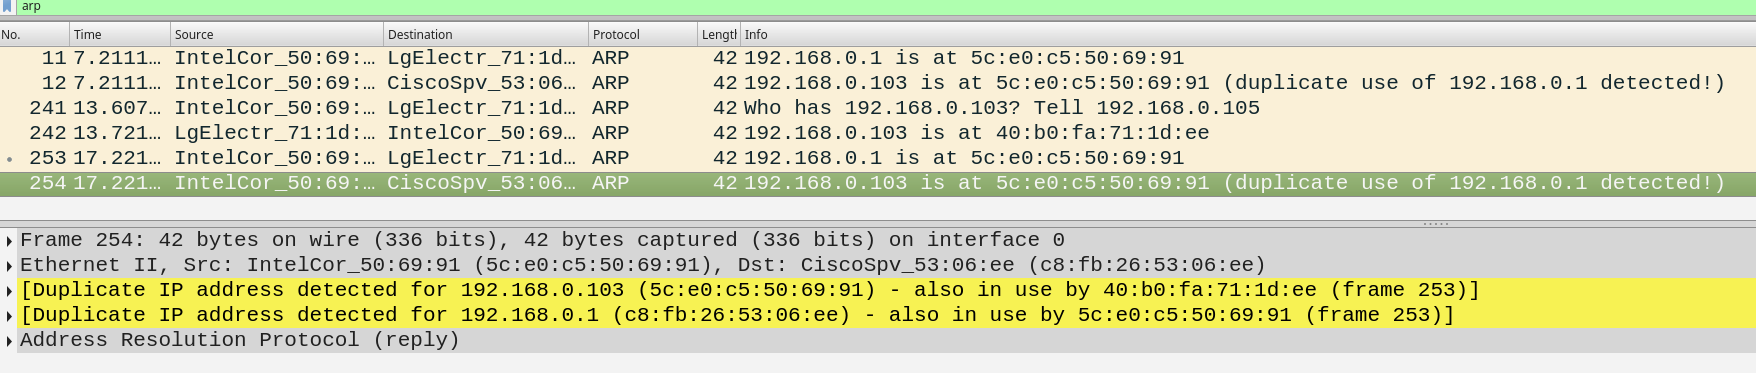
\includegraphics[width=450px]{arppoisoninaction.png}

In this assignment I used ettercap to ARP poison and wireshark to capture the packets. I used Will's website \href{http://williamsigouin.xyz/}{Link} for a non-SSL website, and mine, \href{https://notturing.ddns.net/tyler/IS_ASS2/form.php}{Link} for a website with SSL.

\section*{Packet Output}

Wireshark Configuration:\\
Capture Filter: host 192.168.0.103 (the ip of my phone)\\
Display Filter: http.request.method == GET or http.request.method == POST\\
\\
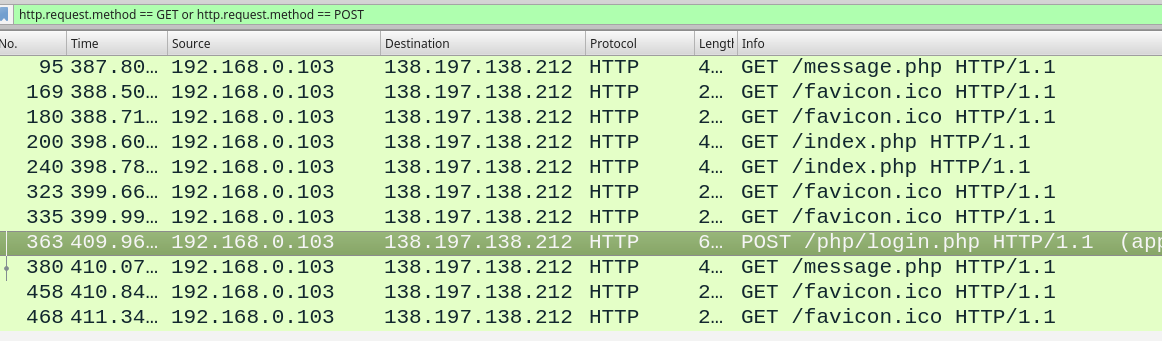
\includegraphics[width=450px]{arppoison.png}
\\
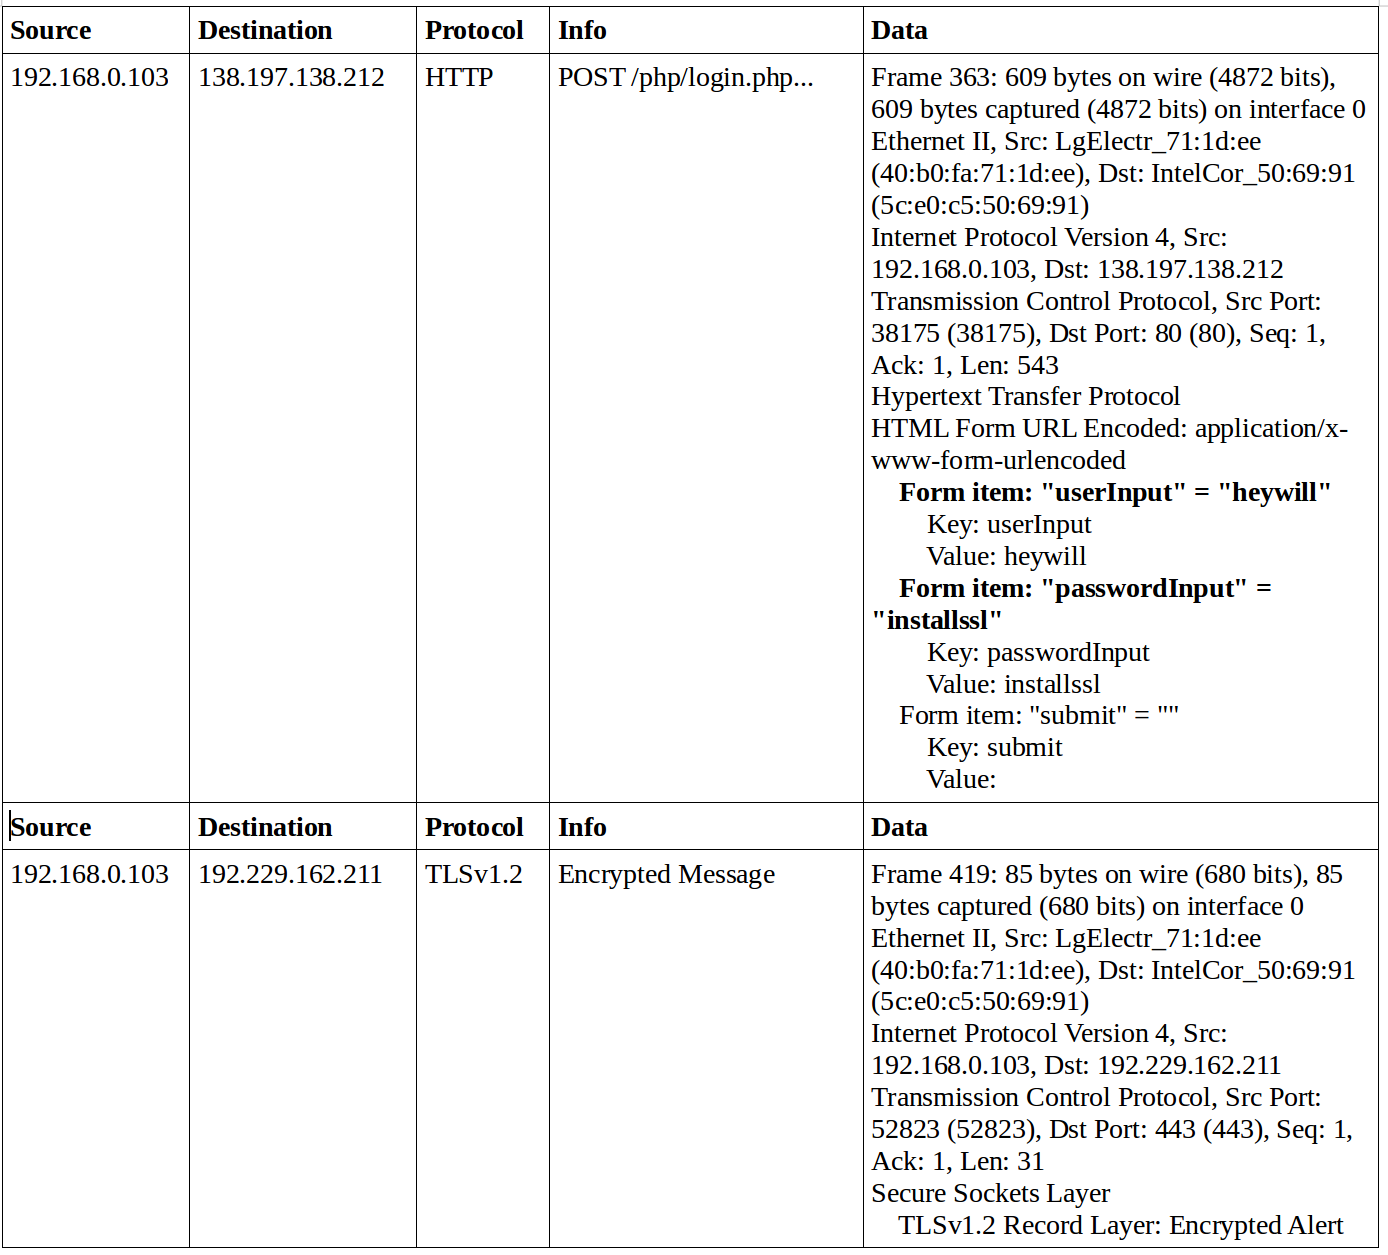
\includegraphics[width=450px]{packetoutput.png}
\\
As we can see with the above results, the non-SSL website has all its data sent unencrypted through the HTTP protocol, but the SSL secured website has everything encrypted over the Secure Socket Layer protocol and no data is available.

\end{document}
